\documentclass{article}

%%%%%%%%%%%%%%%%%%%%%%%%%%%%%%%%%%%%%%%%%%%%%%%%%%%%%%%%%%%%%%%%%%%%%%%%%%%%%%%%
% German language settings. Allows the use of umlauts.                         %
%%%%%%%%%%%%%%%%%%%%%%%%%%%%%%%%%%%%%%%%%%%%%%%%%%%%%%%%%%%%%%%%%%%%%%%%%%%%%%%%
\usepackage[utf8]{inputenc}
\usepackage[T1]{fontenc}
\usepackage[ngerman]{babel}

%%%%%%%%%%%%%%%%%%%%%%%%%%%%%%%%%%%%%%%%%%%%%%%%%%%%%%%%%%%%%%%%%%%%%%%%%%%%%%%%
% These packages provide fonts for the document, but may require manual        %
% installation. The usual procedure (on Linux) is the following:               %
% 1. Download the package files                                                %
% 2. Extract the files to ~/texmf/tex/latex/newpackage                         %
% 3. If never done before, run "texhash ~/texmf" in a terminal                 %
% 4. run "sudo texhash" in a terminal                                          %
%                                                                              %
% At least one of these fonts is most likely available on your system. If this %
% is not the case, you can simply comment all package imports to use the       %
% default font "Computer Modern Roman".                                        %
%%%%%%%%%%%%%%%%%%%%%%%%%%%%%%%%%%%%%%%%%%%%%%%%%%%%%%%%%%%%%%%%%%%%%%%%%%%%%%%%

% TeX Gyre Times 
\usepackage{tgtermes}

% Fourier Font
% \usepackage{fourier}

% A somewhat outdated Times alternative
% \usepackage{mathptmx}

% A Palatino substitute with adjusted line spreading.
% \usepackage{mathpazo}
% \linespread{1.05}

%%%%%%%%%%%%%%%%%%%%%%%%%%%%%%%%%%%%%%%%%%%%%%%%%%%%%%%%%%%%%%%%%%%%%%%%%%%%%%%%
% This package provides the useful commands \set and \Set, that can be used to %
% denote sets. The \set command uses rigid brackets, whereas the \Set command  %
% employs flexible brackets to enclose the set.                                %
% Examples:                                                                    %
%  A \setminus \set{a_0}                                                       %
%  \set{x \in A | x \le 4}                                                     %
%  \Set{\int_{\Omega} f d\mu | f \in \mathcal{L}_2(\Omega, \mathfrak{A}, \mu)} %
%%%%%%%%%%%%%%%%%%%%%%%%%%%%%%%%%%%%%%%%%%%%%%%%%%%%%%%%%%%%%%%%%%%%%%%%%%%%%%%%

\usepackage{braket}

%%%%%%%%%%%%%%%%%%%%%%%%%%%%%%%%%%%%%%%%%%%%%%%%%%%%%%%%%%%%%%%%%%%%%%%%%%%%%%%%
% Several packages for mathematical symbols.                                   %
%%%%%%%%%%%%%%%%%%%%%%%%%%%%%%%%%%%%%%%%%%%%%%%%%%%%%%%%%%%%%%%%%%%%%%%%%%%%%%%%

\usepackage{amsmath, amsfonts, amssymb}

%%%%%%%%%%%%%%%%%%%%%%%%%%%%%%%%%%%%%%%%%%%%%%%%%%%%%%%%%%%%%%%%%%%%%%%%%%%%%%%%
% Provides double-stroked black board letters. In general \mathbb{LETTER is    %
% preferrable, but this package also provides a double-stroked 1: mathds{1}.   %
%%%%%%%%%%%%%%%%%%%%%%%%%%%%%%%%%%%%%%%%%%%%%%%%%%%%%%%%%%%%%%%%%%%%%%%%%%%%%%%%

% \usepackage{dsfont}

%%%%%%%%%%%%%%%%%%%%%%%%%%%%%%%%%%%%%%%%%%%%%%%%%%%%%%%%%%%%%%%%%%%%%%%%%%%%%%%%
% This package provides theorem-like environments.                             %
%%%%%%%%%%%%%%%%%%%%%%%%%%%%%%%%%%%%%%%%%%%%%%%%%%%%%%%%%%%%%%%%%%%%%%%%%%%%%%%%

\usepackage{amsthm}

%%%%%%%%%%%%%%%%%%%%%%%%%%%%%%%%%%%%%%%%%%%%%%%%%%%%%%%%%%%%%%%%%%%%%%%%%%%%%%%%
% Theorem environments, use "thm" for italic fonts inside theorem environments %
% and "def" for normal fonts. These differ from the originals: newline is      %
% created after the complete name (including optional parenthesis) of the      %
% theorem.                                                                     %
%%%%%%%%%%%%%%%%%%%%%%%%%%%%%%%%%%%%%%%%%%%%%%%%%%%%%%%%%%%%%%%%%%%%%%%%%%%%%%%%
 
\newtheoremstyle{thm}       % name
    {15pt}                  % Space above
    {10pt}                  % Space below
    {\itshape}              % Body font
    {}                      % indent amount
    {\bf}                   % Theorem head font
    {}                      % Punctuation after theorem head
    {\newline}              % space after theorem head
    {}                      % Theorem head spec

\newtheoremstyle{def}
    {15pt}
    {10pt}
    {}
    {}
    {\bf}
    {}
    {\newline}
    {}

%%%%%%%%%%%%%%%%%%%%%%%%%%%%%%%%%%%%%%%%%%%%%%%%%%%%%%%%%%%%%%%%%%%%%%%%%%%%%%%%
% The following commands provide enumeration features that yield a section-    %
% based numbering, which is continous through all defined environments. This   %
% is achieved by anchoring one environment to the section numbering. All       %
% subsequent environment are numbered in the same fashion as the single one.   %
%%%%%%%%%%%%%%%%%%%%%%%%%%%%%%%%%%%%%%%%%%%%%%%%%%%%%%%%%%%%%%%%%%%%%%%%%%%%%%%%

\swapnumbers

\theoremstyle{thm}

\newtheorem{intTheorem}{Satz}[subsection]             % Theorem
\newtheorem{intCorollary}[intTheorem]{Korollar}    % Corollary
\newtheorem{intLemma}[intTheorem]{Lemma}           % Lemma

\theoremstyle{def}
\newtheorem{intDefinition}[intTheorem]{Definition} % Definition

%%%%%%%%%%%%%%%%%%%%%%%%%%%%%%%%%%%%%%%%%%%%%%%%%%%%%%%%%%%%%%%%%%%%%%%%%%%%%%%%
% Actual environments. The parameters are:                                     %
% #1 - name of the block (e.g. term to be defined)                             %
% #2 - label of the block (purely for internal reference purposes)             %
%%%%%%%%%%%%%%%%%%%%%%%%%%%%%%%%%%%%%%%%%%%%%%%%%%%%%%%%%%%%%%%%%%%%%%%%%%%%%%%%

\newenvironment{theorem}[2] % 1=Name, 2=Label
  {\begin{intTheorem}[#1] 
   \label{#2}
   %\addcontentsline{toc}{section}{\protect\numberline{\ref{#2}} #1}
   } 
  {\end{intTheorem}}

\newenvironment{corollary}[2] % 1=Name, 2=Label
  {\begin{intCorollary}[#1]
   \label{#2}
   %\addcontentsline{toc}{section}{\protect\numberline{\ref{#2}} #1}
   }
  {\end{intCorollary}}

\newenvironment{lemma}[2] % 1=Name, 2=Label
  {\begin{intLemma}[#1]
   \label{#2}
   %\addcontentsline{toc}{section}{\protect\numberline{\ref{#2}} #1}
   } 
  {\end{intLemma}}
 
\newenvironment{definition}[2] % 1=Name, 2=Label
  {\begin{intDefinition}[#1]
   \label{#2}
   %\addcontentsline{toc}{section}{\protect\numberline{\ref{#2}} {#1}}
   }
  {\end{intDefinition}}


\usepackage{enumerate}
\usepackage{wrapfig}
\usepackage{listings}
\usepackage{color}
\usepackage{enumitem}
\usepackage{graphicx}
\usepackage{float}

\setlist[itemize,2]{label=$\circ$} %nur blubbel für aufzählung zweiter-stufe
\setlist[itemize]{itemsep=1pt} % geringerer abstand zwischen items

\newcommand{\vampire}{\textsc{Vampire}~} 
\newcommand{\proverNine}{\textsc{Prover}9~} 

\makeatletter %definition of classes for highlighting
\lst@InstallKeywords k{tfftypes}{tfftypesstyle}\slshape{tfftypesstyle}{}ld
\lst@InstallKeywords k{tfffunctions}{tfffunctionsstyle}\slshape{tfffunctionsstyle}{}ld
\lst@InstallKeywords k{formulatypes}{formulatypesstyle}\slshape{formulatypesstyle}{}ld
\lst@InstallKeywords k{tptpkeywords}{tptpkeywordsstyle}\slshape{tptpkeywordsstyle}{}ld
\lst@InstallKeywords k{roles}{rolesstyle}\slshape{rolesstyle}{}ld
\makeatother

% Define Language for highlighting
\lstdefinelanguage{tptp}
{
	% list of keywords
	tfftypes={
		\$tType,
		\$i,
		\$o,
		\$int,
		\$rat,
		\$real,
		\$array1,
		\$array2,
	},
	formulatypes={
		fof,
		tff,
		cnf,
		tpi,
		thf,
		bnf,
	},
	tfffunctions={
		\$sum,		\$product,
		\$difference,
		\$uminus,
		\$torat,
		\$toreal,
		\$less,
		\$lesseq,
		\$greater,
		\$greatereq,
	},
	tptpkeywords={
		\$ite\_f,
		\$ite\_t,
		\$let\_tt,
		\$let\_tf,
		\$let\_ft,
		\$let\_ff,
	},
	roles={
		axiom,
		hypothesis,
		conjecture,
		type,
	},	
	keywords={ %add more for highlighting of in formula defined functions
		member, 
		sum,
		even,
		divides,
		pyth,
		primPyth,
	},
	sensitive=true, % keywords are case-sensitive
	morecomment=[l]{\%}, % l is for line comment
	morecomment=[s]{/*}{*/}, % s is for start and end delimiter
	%morestring=[b]" % defines that strings are enclosed in double quotes
}

% Define Colors for highlighting
\usepackage{color}
\definecolor{blue}{RGB}{0,0,205}
\definecolor{lightblue}{RGB}{99,184,255}
\definecolor{green}{RGB}{0,139,0}
\definecolor{purple}{RGB}{139,0,139}
\definecolor{red}{RGB}{205,38,38}
\definecolor{orange}{RGB}{205,102,0}
\definecolor{brown}{RGB}{139,69,19}
\definecolor{grey}{RGB}{160,160,160}

% Set Language for highlighing
\lstset{
	language={tptp},
	basicstyle=\small\ttfamily, % Global Code Style
	captionpos=b, % Position of the Caption (t for top, b for bottom)
	extendedchars=true, % Allows 256 instead of 128 ASCII characters
	tabsize=2, % number of spaces indented when discovering a tab 
	columns=fixed, % make all characters equal width
	keepspaces=true, % does not ignore spaces to fit width, convert tabs to spaces
	showstringspaces=false, % lets spaces in strings appear as real spaces
	breaklines=true, % wrap lines if they don't fit
	frame=trbl, % draw a frame at the top, right, left and bottom of the listing
	frameround=tttt, % make the frame round at all four corners
	numbers=left, % show line numbers at the left
	numberstyle=\tiny\ttfamily, % style of the line numbers
	commentstyle=\color{grey}, % style of comments
	%stringstyle=\color{missing_color}, % style of strings
	tfftypesstyle=\color{lightblue}, % style of tff-types (e.g. $int)
	formulatypesstyle=\color{purple}, % style of foruma-types (e.g. fof)
	tfffunctionsstyle=\color{orange}, % style of tff-functions (e.g. $sum)
	tptpkeywordsstyle=\color{green}, % style of tptp-keywords (e.g. $ite_f)
	rolesstyle=\color{brown}, % style of roles (e.g. axiom)
	keywordstyle=\color{blue}, %style of general keywords like introduced functions (e.g. member)
}

\author{
	Maximilian Reinhart\\
	Martin Bittermann
}

\title{\vampire: Grundlagen und Anwendung}

% Generate PDF hyperlinks when referencing sections and stuff. 
\usepackage{hyperref}

% Frakturzeichen -  Double-stroke symbols
\usepackage{dsfont}

\begin{document}

\maketitle

%%%%%%%%%%%%%%%%%%%%%%%%%%%%%%%%%%%%%%%%%%%%%%%%%%%%%%%%%%%%%%%%%%%%%%%%%%
\begin{abstract}
	Dieser Artikel verschafft zunächst ein grundlegendes Verständnis über den automatischen Theorembeweiser \vampire und
	stellt den Bezug zu ~\cite{cav2013} her. \\
	Es wird eine Einführung in die generelle Benutzung der Software und die verwendete Problembeschreibungssprache, TPTP, gegeben, 
	die Funktionsweise und einige ausgewählte Algorithmen erklärt und
	die Ausgabe von \vampire sowohl analysiert als auch graphisch dargestellt.
	Es werden Parallelen zu anderen Theorembeweisern aufgezeigt, \vampire mit diesen verglichen 
	und zum Schluss wird mit Hinblick auf mögliche Anwendungsbereiche ein Fazit und ein Ausblick gegeben.
\end{abstract}


%%%%%%%%%%%%%%%%%%%%%%%%%%%%%%%%%%%%%%%%%%%%%%%%%%%%%%%%%%%%%%%%%%%%%%%%%%
\section{Einleitung}
\label{sec:introduction}
Automatische Theorembeweiser (ATP) versuchen ohne Benutzerinteraktion Aussagen über gegebene Formeln durch Anwendung von Regeln und Axiomen, die ihnen vorliegen, zu beweisen.
Hierfür wird das Problem von Hand in eine formale Struktur gebracht, die der Beweiser verarbeiten kann.
Diese Formalisierung stellt auch für triviale Probleme eine gefährliche Fehlerquelle dar. 
Nichtsdestotrotz ist für komplexe Probleme das Formalisieren einfacher als das Beweisen per Hand und nach korrekter Formalisierung liefert der ATP mit etwas Glück, nach vertretbarer Zeit,
einen formal korrekten Beweis. Scheitert der Beweis an Zeit- oder Speicherlimits, kann eine
Umformulierung oder Aufteilung in kleinere Probleme helfen, dies bringt eine interaktive
Komponente in das automatische Theorembeweisen.
Anwendung finden ATP in vielerlei Gebieten, unter anderem Hardwaredesign und -verifikation, Softwareverifikation, wissensbasierte Systeme und klassische mathematische Problemstellungen.
Der Vorteil von ATP liegt in diesen Gebieten in der Fähigkeit, Probleme zu bearbeiten, 
die für eine manuelle Beweisführung (teils um Größenordnungen) zu umfangreich sind.
\vampire ist ein ATP für Logik erster Stufe (Prädikatenlogik) mit Gleichheit. Die erste Implementierung stammt von 1993, im Verlauf wurde die Software mehrfach um- und neugeschrieben.
Die Software umfasst heute etwa 152,000 SLOC in C++ und wurde hauptsächlich von Andrei Voronkov und Kry{\v{s}}tof Hoder an der University of Manchester entwickelt.
Neuere Entwicklungen und Ideen stammen vemehrt von Laura Kov{\'a}cs und Ioan Dragan, der Arbeiten am SAT-Beweiser und der Bound Propagation übernommen hat.
Derzeit wird an der vierten Version von \vampire gearbeitet.
\vampire hat dreißig Preise gewonnen und seit 1999 in der Weltmeisterschaft für automatische Theorembeweiser (CASC) jedes Mal mindestens in einer Kategorie gewonnen.
Insgesamt zwölf Mal hat er bei der CASC die Kategorie für Logik erster Stufe gewonnen und elf Mal für CNF/MIX. ~\cite{vampirehp} \\ Daher gilt \vampire allgemein hin als sehr schnell.
Dank seiner Multiplattform- und Multicore-Unterstützung soll er auf allen gängigen Betriebssystemen, wie Linux, Windows und Mac eingesetzt werden können und mehrere Beweisversuche gleichzeitig bearbeiten können.
Wir vermögen zu bestätigen, dass die uns vorliegende Version 3.0 auf Windows 7, 64-bit funktioniert, lediglich mehrere Kerne wurden nicht benutzt und somit nicht mehrere Beweisversuche parallel unternommen.
\vampire löst Probleme über die ihm über die Kommandozeile mitgegebene Strategie, die über den Mode-Befehl eingestellt werden kann und besitzt eine auf einzigartige limited resource strategy, die für kurze Zeitlimits sehr effizient sein soll. Mit \vampire ist es, neben seiner Funktion als ATP, auch möglich ein Expertensystem zu betreiben, das auf Grund von gegebenen Aussagen Antworten aus einer Wissenssammlung geben kann, ebenso ist \vampire zur Programmverifikation für C-Programme mit Schleifen geeignet. 
Leider steht \vampire entgegen der Aussage in ~\cite{cav2013} nicht unter einer liberalen Lizenz, sondern unter einer nicht-freien, proprietären Lizenz, die in ~\cite{vampirehp} einzusehen ist.
Als Primärquelle für diese Arbeit dient der Artikel \textit{First-Order Theorem Proving and \vampire}~\cite{cav2013}.
Weitere Informationen stammen aus \textit{Interpolation and Symbol Elimination in \vampire}~\cite{hoder2010} 
und \textit{Finding Loop Invariants for Programs over Arrays Using a Theorem Prover}~\cite{kovacs2009finding}.
Die Arbeit ist praxisorientiert und kann als Einstiegstutorial verwendet werden.
In dieser \hyperref[sec:introduction]{Einleitung} wurden Grundlagen über automatische Theorembeweiser vermittelt, die einen schnellen Einstieg in das Thema ermöglichen.\\
Als Vorbereitung für die Benutzung von \vampire wird auf die Syntax und Semantik der von \vampire verwendeten \hyperref[sec:input]{Problembeschreibungssprache TPTP} eingegangen. Es werden Hilfestellungen zur Formulierung von Axiomen und Problemen gegeben, sowie Erweiterungen der Sprache durch \vampire dargelegt.
Mit dieser Grundlage wird die \hyperref[sec:invocation]{Benutzung von \vampire}, insbesondere der Aufruf des Programms und die vielen einstellbaren Optionen behandelt.\\
Anschließend wird die \hyperref[sec:mechanics]{Funktionsweise} von \vampire in den Grundzügen erklärt und das zugrunde liegende Beweisverfahren mit einigen ausgewählten Algorithmen erläutert.\\
Schließlich folgt eine Veranschaulichung der \hyperref[sec:output]{Beweisausgabe}. \\
Ein kurzes \hyperref[sec:conclusion]{Schlusswort} schließt die Arbeit ab.



%%%%%%%%%%%%%%%%%%%%%%%%%%%%%%%%%%%%%%%%%%%%%%%%%%%%%%%%%%%%%%%%%%%%%%%%%%
\section{TPTP Eingabe}
\label{sec:input}

TPTP ist die Sprache, in der Probleme und Axiome geschrieben sein müssen, damit \vampire sie bearbeiten kann. TPTP besitzt Ähnlichkeit zu Prolog und wird von vielen heutigen Theorembeweisern für Logik 1. Stufe unterstützt. \cite[S. 4]{cav2013}. Die Sprache dient als Grundlage für die gleichnamige \textit{Thousands of Problems for Theorem Provers (TPTP)} Bibliothek.~\cite{tptphp} Die Sprache unterstützt unter anderem folgende Formeltypen:
\begin{itemize}
	\item First order formula (FOF)
	\item Typed first order formula (TFF)
	\item Clause normal form (CNF)
	\item TPTP Process Instruction Language  (TPI)
	\item Typed higher order form (THF)
\end{itemize}
Die wichtigsten, die von \vampire unterstützten werden, sind FOF, TFF und CNF.

\subsection{Syntax}
\label{subsec:syntax}
\begin{wraptable}{r}{4cm}
\begin{tabular}{|c|c|}
	\hline TPTP & Bedeutung \\ 
	\hline \$false & $\bot$\\
	\hline \$true & $\top$\\
	\hline ?[X]: & $\exists$X: \\
	\hline ![X]: & $\forall$X: \\
	\hline = & = \\
	\hline != & $\neq$ \\
	\hline $\sim$ & $\lnot$ \\
	\hline | & $\lor$ \\
	\hline \& & $\land$ \\
	\hline => & $\Rightarrow$ \\
	\hline <=> & $\Leftrightarrow$ \\
	\hline Y & Variable \\
	\hline y & Literal \\
	\hline f(x, A, B) & Prädikat \\
	\hline \% \dots & Kommentar \\
	\hline
\end{tabular} 
\end{wraptable}
Eine Datei im TPTP-Format besteht aus Formeln, include-Statements und Kommentaren.
Eine Formel in TPTP beginnt stets mit der Information über ihren Typ. Hierbei können zum Beispiel \texttt{fof(...), tff(...), cnf(...)} und einige mehr verwendet werden.
Innerhalb der Klammern werden drei Bereiche unterschieden, die jeweils mit einem Komma voneinander getrennt sind. 
Der erste Parameter is der Name der Formel, beginnend mit einem kleinen Buchstaben [a-z], welcher lediglich zur besseren Übersicht im späteren Beweis verwendet wird und ansonsten weder benutzt wird noch eindeutig sein muss.
Zweiter Parameter ist die Rolle, die diese Formel einnimmt, hierbei kann es sich um ein Axiom (\texttt{axiom}), eine Hypothese (\texttt{hypothesis}) oder eine Behauptung (\texttt{conjecture}) handeln.
Eine Rolle ist eine wichtige Voraussetzung für den Beweiser, denn hierdurch erfährt er, welche Grundvoraussetzungen und Annahmen getroffen wurden, die er als richtig behandeln kann um die gestellte Behauptung zu beweisen.
In einer Problemdatei sollte nur eine einzige Behauptung stehen, denn sobald \vampire einen Beweis zu einer der gegebenen Behauptungen gefunden hat, gibt er diesen aus und bricht die Arbeit an den anderen ab.
Letztendlich steht im dritten Teil die Formel in der Anfangs gewählten Syntax, die der Beweiser behandeln kann. \cite[S. 4-5]{cav2013}
\subsection{First order formula (FOF)}
\label{subsec:tptpfof}
\[\forall X,A : X \in \bigcup A \Leftrightarrow \exists Y : Y \in A \land X \in Y\]
Möchten wir diese Formel in TPTP umwandeln,
so bedarf es der Definition der Operatoren $\in$ und $\bigcup$, welche in der Syntax von TPTP 
nicht vorhanden sind.
Ein Prädikat kann ohne vorherige Deklaration einfach in einer oder mehreren Formeln 
verwendet werden. 
Die Definition erfolgt über die in jenen Formeln festgelegten logischen Eigenschaften gegenüber 
anderen Prädikaten oder Funktionen. Diese Art der Definition findet sich auch in anderen
Logikprogrammiersprachen.
Ein Axiom kann daher mehrere Prädikate definieren und die Definition eines Prädikats kann 
auf mehrere Axiome verteilt sein.
Im Verlauf des Beweises sucht \vampire nach Möglichkeiten aus den gegebenen Axiomen und Hypothesen Schlüsse und Herleitungen zu ziehen.
So kann die obige Formel in TPTP formuliert werden:
\begin{lstlisting}[language=tptp]
! [X,A] : (member(X,sum(A))
	<=> ? [Y] : (member(Y,A) & member(X,Y)).
\end{lstlisting}
$\in$ wurde durch \verb=member(...)= ersetzt, $\bigcup$ durch \verb=sum(...)=.
Legen wir jetzt fest, dass es sich um Logik erster Stufe handelt (\textit{fof(...)}), dass die Definition, 
die Namensgeber wird, da wir diese vorwiegend tätigen, die große Vereinigung über eine Menge ist (sum) und, dass es sich um ein \textit{axiom} handelt,
entsteht in Verbindung mit unser umgewandelten TPTP-Formel folgende fertige TPTP-Aussage:
\begin{lstlisting}[language=tptp]
fof(Sum, axiom, (	
	! [X,A] : (member(X, sum(A)) 
		<=> ? [Y] : (member(Y, A) & member(X, Y))))).
\end{lstlisting}
Eine solcher Block wird immer mit einem Punkt abgeschlossen.
Zusätzlich mit diesem und anderen Axiomen, die es nutzen, ist das \verb=member=-Prädikat definiert.
Über den Befehl \verb|include(...)| können Dateien, wie zum Beispiel eine Datei mit vorgefertigten Axiomen, in die TPTP-Problem-Datei eingebunden werden. \cite[S. 4-5]{cav2013}

\subsection{Typed first order formula (TFF)}
\label{subsec:tptptff}

\texttt{Tff} ist äquivalent zu \texttt{fof} aufgebaut, doch können hier getypte Variablen verwendet werden. Um eine Variable zu typen muss ihr bei ihrer Verwendung im Quantor mit einem Doppelpunkt ein Typenausdruck, eine \textit{sort}, folgen. \\
Typenausdrücke sind: \begin{itemize}
	\item \verb=$i=: individuell. Standard-Typ, wenn nichts angegeben
	\item \verb=$o=: Boolesch
	\item \verb=$int=: Integer
	\item \verb=$rat=: Rational
	\item \verb=$real=: Reell
	\item \verb=$array1=: Integer-Array
	\item \verb=$array2=: Array von Integer-Array
\end{itemize}
wobei die letzten beiden spezifisch von \vampire definiert sind und nicht im TPTP-Standard verankert sind.
Um besser mit ganzen, reellen oder rationalen Zahlen arbeiten zu können, beinhaltet \vampire folgende, im TPTP-Standard definierten Funktionen, die in \texttt{tff} verwendet werden können:
\begin{itemize}
	\item \verb=$sum=: Addition $(x + y)$
	\item \verb=$product=: Multiplikation $(x * y)$
	\item \verb=$difference=: Differenz $(x - y)$
	\item \verb=$uminus=: einstelliges Minus $(-x)$
	\item \verb=$to_rat=: Konvertierung zu rationalen Zahlen
	\item \verb=$to_real=: Konvertierung zu reellen Zahlen
	\item \verb=$less=: kleiner als $(x < y)$
	\item \verb=$lesseq=: kleiner-gleich $(x \leq y)$
	\item \verb=$greater=: größer als $(x > y)$
	\item \verb=$greatereq=: größer-gleich $(x \geq y)$ 
\end{itemize}
Beispiel: $(x + y) \geq 0$ mit x, y aus den ganzen Zahlen
\begin{lstlisting}[language=tptp]
tff(example,conjecture, 
	? [X:$int,Y:$int] : $greatereq($sum(X,Y),0)).\end{lstlisting} \cite[S. 24-25]{cav2013}
	
{%%%%%da keine gute Möglichkeit eigene Typen zu verwenden oder hinreichend zu erklären bis auf weiteres gestrichen.%%%%%
\iffalse  
Möchte man eigene Typen definieren, ist dies ebenfalls möglich:
\begin{lstlisting}[language=tptp]
tff(own_type,type,own: $tType).
\end{lstlisting}
Der Name, hier \verb|own_type|, kann wie bekannt frei gewählt werden und das Wort \textit{type} ist die Deklaration, dass es sich um eine Typendefinition handelt, wobei dieses Wort sowohl uneindeutig als auch redundant ist.
Zuletzt wird \verb|own|, der eigentliche Typname, der auch frei gewählt werden kann, angegeben und mit dem angefügten \verb|$tType| als neuer Typ definiert.
Nachfolgend gezeigt ist die Typdefinition eines Literals a des Typs \verb|own| und einer Funktion f, die zwei Argumente übernimmt, deren Typen \verb|own| sind, und deren Ausgabe wieder des Typs \verb|own| ist.\\
\begin{lstlisting}[language=tptp]
tff(a_has_type_own,type,a : own).
tff(f_has_type_own,type,f : own * own > own).
\end{lstlisting}

\fi 
} % Ende der streichung

%%%%%%%%%%%%%%%%%%%%%%%%%%%%%%%%%%%%%%%%%%%%%%%%%%%%%%

{%%%%%if-then-else und let...in bis auf weiteres gestrichen%%%%%
\iffalse 
\subsection{If-Then-Else}
\label{subsec:tptpitef}

Vereinfachend für die Programmverifikation kann beim umschreiben von Programmen nach TPTP das if-then-else-Konstrukt \verb=$ite_f= für Formeln und \verb=$ite_t= für Terme benutzt werden.
\begin{lstlisting}[language=tptp]
$ite_f(Bedingung, Dann, Sonst) % aequivalent fuer $ite_t
\end{lstlisting}
\begin{lstlisting}[language=tptp]
tff(c1,axiom,((($ite_f(p & q, ~p | ~q, p & q)).
tff(c2,axiom,($ite_t(p,a,b) != (a & p)).
\end{lstlisting}
~\cite{hoder2011slides}
\subsection{Let...in}
\label{subsec:tptpletin}

Gleichsam kann das $let\dots in$-Konstrukt für für Therme \verb=$let_tt=, für Formeln \verb=$let_ff=, und zwischen Thermen und Formeln, bzw. Formeln und Thermen \verb=$let_tf= und \verb=$let_ft= verwendet werden.
\begin{lstlisting}[language=tptp]
tff(c1,axiom,
	$let_tt(f(X), g(X), f(a)) != g(a)).
tff(c2,axiom,
	$let_ff}(p(X), q(X) | r(X), p(c)) & ~q(c) & ~r(c)).
tff(c3,axiom,
	$let_tf(f(X), g(X), p(f(X))) & ~p(g(X))).
tff(c4,axiom,
$let_ft(p(X), q, $ite_t(p(a), a, b)) != $ite_t(q, a, b)).
\end{lstlisting}

\fi % ende der streichung
}

\subsection{Beispiel}
\label{subsec:tptpexample}

Mit den TFF-Formeln und \vampire's Axiomatisierung der ganzen Zahlen können wir nun 
ein einfaches Problem aus dem Gebiet der Zahlentheorie formulieren.

\begin{definition}{Pythagoreisches Tripel}{def:pythtrip}
	Ein Tripel $(x, y, z) \in \mathds{N}^3$ ist ein pythagoreisches Tripel, wenn
	$x^2+y^2=z^2$ gilt.
\end{definition}
\begin{definition}{Primitives pythagoreisches Tripel}{def:primpythtrip}
	Ein pythagoreisches Tripel $(x, y, z)$ heißt \emph{primitiv}, falls x, y und z teilerfremd sind.
\end{definition}
Folgenden Satz möchten wir beweisen:
\begin{theorem}{}{thm:oddHyp}
	Für jedes primitive pythagoreische Tripel $(x, y, z)$ gilt: $z$ ist ungerade.
\end{theorem}
Aus Definition \ref{def:pythtrip} lässt sich mit den eingebauten Funktionen direkt ein Prädikat schreiben, das bestimmt ob ein gegebenes Tripel aus ganzen Zahlen ein pyth. Tripel ist.
Für Definition \ref{def:primpythtrip} benötigen wir hilfsweise ein teilt-Prädikat.
Schließlich lässt sich der Satz \ref{thm:oddHyp} als Behauptung formulieren. 
Eine Hypothese-Formel benötigen wir nicht, da der Satz unter den gegebenen Axiomen allgemeingültig sein sollte.
\begin{lstlisting}[language=tptp]
% even-Praedikat: X ist gerade
tff(even, axiom, ![X:$int] : (even(X) =>
(?[Y:$int] : ($product(Y,2) = X)))).

% Teilbarkeits-Praedikat: X teilt Y <=> es ex. Z mit Z*X = Y
tff(divides, axiom, (![X:$int,Y:$int] : (divides(X,Y) <=>
   (?[Z:$int] : $product(Z,X) = Y)))).

% pyth-Praedikat: X,Y,Z ist pyth. Tripel mit Z Hypotenuse
tff(pyth, axiom, ![X:$int,Y:$int,Z:$int] : (pyth(X,Y,Z)
   <=> ($sum($product(X,X),$product(Y,Y))=$product(Z,Z)))).

% Primitives-Pyth.-Tripel Praedikat
tff(primPyth, axiom, (![X:$int,Y:$int,Z:$int] : 
   primPyth(X,Y,Z) <=> (pyth(X,Y,Z) & (~?[D:$int]: 
   ($product(D,D) != 1) & divides(D,X) & divides(D,Y) & 
   divides(D,Z))))).

% Behauptung: Die Hypotenuse jedes primitiven 
% pythagoreischen Tripels ist ungerade.
tff(oddHyp, conjecture, (![X:$int,Y:$int,Z:$int] : 
   primPyth(X,Y,Z) => ~even(Z))).
\end{lstlisting}
Das Problem speichern wir in der Datei \verb|pytrip.p|.

%%%%%%%%%%%%%%%%%%%%%%%%%%%%%%%%%%%%%%%%%%%%%%%%%%%%%%
\section{Benutzung von \vampire}
\label{sec:invocation}
Die grundlegende Benutzung von \vampire ist, wie in \cite{cav2013} behauptet, recht einfach. Nachdem man das Programm vorliegen hat, wird über die Kommandozeile die enthaltene ausführbare Datei gestartet. Nun liest \vampire von \texttt{STDIN}. Der Benutzer kann direkt in der Kommandozeile eine TPTP-Formel eingegeben, die an \vampire übergeben werden soll. Falls diese schon vorgeschrieben in einer Datei vorliegt, kann diese Datei über die jeweilige Shell-Syntax an \vampire übergeben werden. Nachdem \vampire das Problem erhalten hat, beginnt es direkt mit der Arbeit. 
Unter Windows liefert die folgende Kommandozeile den Beweis für das in der \verb|pytrip.p| 
formulierte Problem:\\

\texttt{vampire.exe < pytrip.p}\\\\
Die gesamte Ausgabe kann auch zur späteren Verwendung in die Datei output.txt geschrieben werden:\\

\texttt{vampire.exe < pytrip.p > output.txt}\\\\
In \ref{sec:output} wird auf die Interpretation der Ausgabe eingegangen.

\subsection{Kommandozeilenparameter}
\label{subsec:commands}
\vampire lässt sich hochgradig in seiner Bearbeitung des Problems beeinflussen. Dazu werden dem Aufruf in der Konsole Parameter beigefügt, die in \cite{cav2013} und in \cite[S. 2, 20]{hoder2011slides} aufgeführt sind und von denen nachfolgend einige Ausgewählte genannt werden:
\begin{itemize}	
	\item \verb= --theory_axioms [on|off]= \label{arg:theoryaxiomsoff}\\
	\vampire fügt selbstständig ihm bekannte Axiome über bestimmte \emph{theories}, wie die Arithmetik auf natürlichen Zahlen, hinzu. Standard ist \textit{on}.
	\item \verb=--proof [on|off]= \label{arg:proofoff}\\
	Die Beweisausgabe kann entweder mit vollständigem Beweis oder nur mit einer Aussage über den Ausgang des Beweisversuches geschehen. Standard ist \textit{on}.
	\item \verb|-t X| oder \verb|--time_limit X| \label{arg:timelimit}\\
	\vampire bricht nach X Sekunden den Versuch ab das Problem zu lösen. Sollte bis dahin kein Beweis gefunden worden sein, gibt \vampire \texttt{time limit expired} aus. Standardmäßig liegt das Zeitlimit bei 60  Sekunden.
	\item \verb|-m X oder --memory_limit X| \label{arg:memorylimit}\\
	Dieser Befehl setzt das Speicherlimit auf X in Megabyte. Grundsätzlich nutzt \vampire allen verfügbaren Speicher, den es adressieren kann, was bei 32-bit Binaries weniger als 4GB entspricht.
	\item \verb|--age_weight_ratio X:Y| \label{arg:ageweightratio}\\
	Das Verhältnis von Alter zu Gewicht bestimmt, von welchen der beiden Prioritätsqueues, die \vampire von Klauseln unterhält, wie viele gewählt werden. X und Y müssen ganzzahlige, positive Zahlen sein.
	2:3 würde beispielsweise bedeuten, dass je 2 der ältesten und je 3 der leichtesten Klauseln gewählt werden.  
	\item \verb|--nongoal_weight_coefficient X| \label{arg:weightcoefficient}\\
	Erlaubt das einstellen des Koeffizienten, der das Gewicht einer Klausel bestimmt. Normalerweise ist die Anzahl der Symbole in der Klausel gleichsam das Gewicht.
	\item \verb|--max_weight X| \label{arg:maxweight}\\
	Stellt das ansonsten von \vampire veränderbare maximale Klauselgewicht ein. \vampire kann bei Speicherknappheit oder bei nutzen der \emph{limited resource strategy} das Maximum ansonsten automatisch verringern um schwere Klauseln zu verwerfen.
	\item \verb|--forced_options <option1[:option2[:option3[...]]]>| \label{arg:forcedoptions}
	\begin{itemize}
		\item \verb|propositional_to_bdd=off| \\
		Schaltet das Einführen von Prädikaten für BDD-Variablen aus.
		\item \verb|splitting=off| \\
		Schaltet das Einführen von Prädikaten für Entscheidungspunkte aus.
		
		{ %%%%%da keine ahnung was diese swithes tun, bis auf weiteres gestrichen%%%%
		\iffalse	
		\item \verb|equality_proxy=off|
		\item \verb|general_splitting=off|
		\item \verb|inequality_splitting=0|
		\fi % ende der streichung 
		}
		
		\item \verb|naming=0| \\
		Schaltet Einführen von Prädikaten zur Vermeidung von exponentiellem Ausdehnen während der Klausifizierung aus.
		Standardwert ist 8, je höher die Nummer, desto weniger eingeführte Namen.\\
	\end{itemize}

	\subsubsection{Einstellen des Saturationsalgorithmus}

\item \verb|--saturation_algorithm| \label{arg:saturationalgorithm}
\begin{itemize}
	\item \verb|lrs|\\
	Der standardmäßig gewählte Saturationsalgorithmus von \vampire ist \emph{lrs} (\emph{limited resource strategy}).
	Dieser Algorithmus, der einzigartig in \vampire sein soll, versucht unter den passiven und neuen Klauseln jene zu identifizieren, die niemals in der gegebenen Zeit gelöst werden können und verwirft diese.
	\item \verb|discount|\\
	Diese Art des Algorithmus wurde ursprünglich im \textsc{Discount} System von Jürgen Avenhaus, Jörg Denzinger und Matthias Fuchs implementiert.
	Einen ähnlich arbeitenden Algorithmus verwenden neben \vampire auch \textsc{Waldmeister}, \textsc{E} und \textsc{SPASS}. 
	Die passiven Klauseln, der erzeugten Klauselmenge nehmen nicht am Inferenz- oder Vereinfachungssystem teil.
	\item \verb|otter|\\
	Dieser Art des Algorithmus wurde ursprünglich im OTTER Theorembeweiser von William McCune implementiert.
	Einen ähnlich arbeitenden Algorithmus verwenden neben \vampire auch \textsc{Gandalf} und \textsc{SPASS}. 
	Anders als beim vorherig genannten Algorithmus ist die Teilnahme der passiven Klauseln an der Vereinfachung möglich, wie zum Beispiel, bei Gleichheit der Einheiten, das Neuschreiben oder die Subsumtion. 
\end{itemize}
\cite{cav2013}, \cite[S. 107]{riazanov2003limited}

	\subsubsection{Einstellen des Modus}

\item \verb|-mode <mode>| \label{arg:modes}
Die Angabe eines Modus bestimmt den Ablauf des Beweisprozesses, 
indem die Verwendung einer bestimmten Strategie oder Strategiegemische vorgeben wird.
Einige mögliche Modi sind:
\begin{itemize}
	\item \verb|casc| \\
	Dieser auch bei dem gleichnamigen Wettbewerb verwendete Modus ist laut ~\cite{hoder2011slides} der beste der möglichen Modes.
	Das gegebene Problem wird im Vorfeld analysiert um die Charakteristiken zu erkennen, dann wird es einer von derzeit 43 Klassen zugewiesen. Jede Klasse besitzt eine Abfolge von Strategien, die das Problem lösen sollten.
	Der Mode scheint aber in der von uns verwendeten Version von \vampire nicht lauffähig zu sein (\texttt{sio is not a valid option}).
	\item \verb|casc_ltb| \\
	Dieser Mode wählt die Strategie äquivalent zum normalen casc-Mode. Der Input ist eine Batch-Datei nach den Vorgaben der CASC LTB (Large Theory Batch). Eine Besonderheit um Zeit zu sparen ist das nur einmalige einlesen der Axiome und das anschließende Hinzufügen dieser zu den Problemen denen sie zugewiesen sind. Dieser Mode ist multiprocessing-fähig und kann somit mehrere Strategien parallel verwendet. Dieser Mode wurde von uns nicht getestet.
	\item \verb|axiom_selection| \\
	Sowohl Input als auch Output bei diesem Mode sind Formeln in TPTP oder CNF, wodurch er als Filter fungieren kann, da sein Output von zb. anderen Modes gelesen werden kann.
	Er vollzieht eine Sine-Axiom-Selection, wie in ~\cite{sinquanon} beschrieben.
	\item \verb|clausify| \\
	Dieser Mode konvertiert Formeln von TPTP nach CNF um und unterstützt dabei getypte Formeln, Arithmetik und auch Antwortliterale. Er erlaubt die Anwendung von etlichen Preprocessing rules die \vampire beinhaltet.
	\item \verb|grounding| \\
	Mit diesem Mode wird ein Einstein-Podolsky-Rosen-Paradoxon in ein aussagenlogisches Problem umgewandelt. Der Input erfolgt über TPTP, der Output ist im DIMACS CNF Format.
	Es wird splitting angewendet um die Anzahl der Variablen in den Klauseln und damit die der generierten aussagenlogischen Klauseln gering zu halten.
	\item \verb|consequence_elimination| \\
	Dieser Mode versucht aus einer gegebenen Menge an Behauptungen, der eine Theorie begründet liegen mag, eine der Behauptung aus den anderen herzuleiten.
	\item \verb|bpa| \\
	Bound Propagation (bpa) ersetzt hierbei für das Lösen von lineare Ungleichheiten (quantorenfreie lineare, reelle und rationale Arithmetik) das Superpositionscalculus.
	Dieser Mode ist in unserer Version nicht implementiert.
	\item \verb|program_analysis| \\
	Der letzte hier gezeigte Mode ist für die mit \vampire mögliche Programmverifikation von C-Programmen. Hierbei muss die *.c-Datei an \vampire übergeben werden.
	Dieser Mode wird in unserer Version nicht unterstützt.
\end{itemize}
\end{itemize} % Kommandozeilenoptionen

%%%%%%%%%%%%%%%%%%%%%%%%%%%%%%%%%%%%%%%%%%%%%%%%%%%%%%
%\subsection{Segfaults}
%\label{subsec:segfaults}

%\begin{itemize}
%\item parentheses in input not aligned to magic waves in room
%\item it crash
%\end{itemize}

%%%%%%%%%%%%%%%%%%%%%%%%%%%%%%%%%%%%%%%%%%%%%%%%%%%%%%%%%%%%%%%%%%%%%%%%%%
\section{Funktionsweise}
\label{sec:mechanics}

Dieser Abschnitt gibt einen Einblick in die beweisrelevanten Abläufe, die durch einen typischen Aufruf von \vampire ausgelöst werden, bis zur Ausgabe eines Ergebnisses.

Jedes Problem wird von \vampire nach folgenden Schritten bearbeitet: \cite[S. 9]{cav2013}

\begin{enumerate}
	\itemsep-0.3em 
	\item Lese das Problem
	\item Ermittle die Optionen zur Beweissuche
	\item \emph{Preprocessing}
	\item Konversion in Konjunktive Normalform
	\item Anwendung eines Saturationsalgorithmus
	\item Ausgabe des Resultats mit Beweis oder Gegenbeweis
\end{enumerate}
Dabei nimmt Schritt 5 bei schwierigen Problemen bei weitem die meiste Zeit in Anspruch.

\subsection{Preprocessing}
\label{subsec:preprocessing}

Nachdem \vampire die Eingabe gelesen hat, finden vor der eigentlichen, oft zeitintensiven
Beweissuche einige vorbereitende Schritte statt. Manche dieser Schritte sind Umformungen
auf den eingegebenen Formeln und können in der \hyperref[sec:output]{Beweisausgabe} eingesehen werden.
Diese unvollständige Auflistung enthält einige der ausgeführten Preprocessing-Schritte:

\begin{enumerate}
	\itemsep-0.3em 
	\item Wähle eine \textit{relevante} Teilmenge von Formeln (optional).
	\item Füge Axiome für verwendete Typen (z.B. Integer) hinzu (optional).
	\item Bereinige die Formeln (Bereinigte Normalform).
	\item Sollte eine Formel $\top$ oder $\bot$ beinhalten, \\vereinfache sie.
	\item Entferne if-then-else und let-in Verbindungen.
	\item Ebne die Formeln.
	\item Entferne reine Prädikate.
	\item Entferne nicht genutzte Prädikatdefinitionen \\(optional).
	\item Konvertiere die Formeln in \textit{equivalence negation normal form} (ennf).
	\item Ersetze Subformeln durch ihre Namen.
	\item Konvertiere die Formeln in \textit{negation normal form} (nnf) (optional).
	\item Skolemisiere die Formeln.
	\item Ersetze Gleichheitsaxiome.
	\item Lege eine Ordnung der Literale fest.
	\item Transformiere die Formeln in \textit{conjunctive normal form} (cnf).
	\item Entferne die Funktionsdefinitionen (optional).
	\item Wende \textit{inequality splitting} an (optional).
	\item Entferne Tautologien.
	\item Entferne reine Literale (optional).
	\item Entferne Klauseldefinitionen (optional).
\end{enumerate}

\subsection{Beweis durch Widerspruch}
\label{subsec:refutation}

\vampire beweist Theoreme durch Widerspruch.
Dazu wird die Negation der Behauptung $F$, zusammen mit den Axiomen,
der Formelmenge hinzugefügt.
Nun leitet \vampire durch Inferenz neue Formeln aus den Axiomen und $F$ her, 
mit dem Ziel, die leere Klausel $\bot$ (\texttt{\$false} in TPTP-Schreibweise) zu folgern.
Kann diese hergeleitet werden, ist die gesamte Formelmenge unerfüllbar.
Demzufolge hat die \textit{Negation} der Hypothese unter den angegebenen Axiomen keine Gültigkeit,
im Umkehrschluss ist die Hypothese $F$ bewiesen. \cite[S. 5]{cav2013}\\
Ist die Formelmenge hingegen erfüllbar, kann $\neg F$ aus den Axiomen bewiesen werden.
Damit ist $F$ widerlegt. \cite[S. 7]{cav2013}

%%%%%%%%%%%%%%%%%%%%%%%%%%%%%%%%%%%%%%%%%%%%%%%%%%%%%%
\subsection{Inferenzsystem}
\label{subsec:inference}

Ein Inferenzsystem bildet die Grundlage jeglicher Formelherleitung in \vampire.

\begin{definition}{Inferenzregel}{def:inference}
	Eine Inferenzregel ist eine $n$-stellige Relation auf Formeln, mit $n \leq 0$.
	Es ist üblich diese wie folgt zu schreiben:
	\[F_1  \mathellipsis F_n \over F\]
	$F_1, \mathellipsis , F_n$ bilden dabei die Prämissen, $F$ ist die Konklusion der Regel.
	Axiome sind ein Sonderfall mit $n=0$. Ein Inferenzsystem $\mathds{I}$ ist eine Menge solcher
	Regeln.  \cite[S. 11]{cav2013}
\end{definition}

\vampire implementiert 79 Inferenzregeln. \cite[S. 6]{cav2013}

%%%%%%%%%%%%%%%%%%%%%%%%%%%%%%%%%%%%%%%%%%%%%%%%%%%%%%
\subsection{Saturation}
\label{subsec:saturation}

\vampire als Saturation-basierter Theorembeweiser leitet für eine gegebene Formelmenge $S$
jede unter dem benutzten Inferenzsystem $\mathds{I}$ herleitbare Formel her. Dies stellt die
\emph{Vollständigkeitseigenschaft} des Saturationsalgorithmus dar, d.h. falls $S$ unerfüllbar ist,
dann ist $\bot$ unter $\mathds{I}$ herleitbar. Diese Eigenschaft wird durch eine \emph{faire}
Auswahl an Inferenzen in jedem Saturationsschritt sichergestellt. \cite[S. 12-13]{cav2013}

\begin{definition}{Saturierte Formelmenge}{def:saturatedset}
	Eine Formelmenge $S$ heißt saturiert unter einem Inferenzsystem $\mathds{I}$, wenn für jede $\mathds{I}$-Inferenz mit Prämissen in $S$ die Konklusion ebenfalls in $S$ ist.
\end{definition}

Nach erfolgter Saturation ist die Menge $S$ daher abgeschlossen unter Inferenz, es können
keine neuen Formeln erzeugt werden.
Wird dieser Punkt erreicht, ohne dass $\bot$ hergeleitet wurde, so ist der Beweis gescheitert.

%%%%%%%%%%%%%%%%%%%%%%%%%%%%%%%%%%%%%%%%%%%%%%%%%%%%%%
\subsection{Redundancy Elimination}
\label{subsec:redund}

Ein Saturationsalgorithmus allein führt jedoch nicht zu einem effizienten Beweiser.
Der Suchraum ist zu groß, als dass eine ziellose Inferenzbildung in annehmbaren Zeit- und
Speichergrenzen einen Beweis finden würde.

\vampire eliminiert daher während der Saturation regelmäßig redundante Formeln,
um die Anzahl der aktiven Formel und den daraus resultierenden Suchraum zu verringern.
Eine der einfachsten Kriterien für Redundanz sind Tautologien. 

%%%%%%%%%%%%%%%%%%%%%%%%%%%%%%%%%%%%%%%%%%%%%%%%%%%%%%%%%%%%%%%%%%%%%%%%%%
\section{Beweisausgabe}
\label{sec:output}
Wir greifen hier das Beispiel aus \ref{subsec:tptpexample} wieder auf.
Dies ist ein Ausschnitt der Ausgabe aus der Datei \verb|output.txt|, die wir in \ref{sec:invocation}
erstellt haben:

\begin{verbatim}
Refutation found. Thanks to Tanya!
78. $false (0:0) [sat splitting refutation 77,54,59,49,61,60,76]
...
22. $product(X0,0) = 0 (0:5) [theory axiom]
...
42. ! [X1,X2,X3] : primPyth(X1,X2,X3) & even(sK6) [skolemisation 32]
32. ? [X0] : (! [X1,X2,X3] : primPyth(X1,X2,X3) & even(X0)) [ennf transformation 29]
29. ~! [X0] : (! [X1,X2,X3] : primPyth(X1,X2,X3) => ~even(X0)) [flattening 28]
28. ~! [X0] : (! [X1,X2,X3] : primPyth(X1,X2,X3) => ~even(X0)) [rectify 6]
6. ~! [X2] : (! [X0,X1,X2] : primPyth(X0,X1,X2) => ~even(X2)) [negated conjecture 5]
5. ! [X0,X1,X2] : primPyth(X0,X1,X2) => ~even(X2) [input]
...
------------------------------
Version: Vampire 3.0 (commit unknown)
Termination reason: Refutation

Active clauses: 8
Passive clauses: 33
Generated clauses: 55
...
Memory used [KB]: 127
Time elapsed: 0.008 s
------------------------------
\end{verbatim}

Die Ausgabe von \vampire nach einem erfolgreichen Beweis ist zweigeteilt:
In der ersten Zeile wird durch \verb|Refutation found| angezeigt, dass der 
\emph{Beweis durch Widerspruch} gelungen ist. Danach folgen einige der Formeln, 
die während des Beweises erzeugt wurden. 
Während der Formelerzeugung bekommt jede Formel eine fortlaufende Nummer, beginnend mit den Axiomen und den Eingabeformeln. Wird ein Beweis gefunden, so gibt es einen gerichteten azyklischen Graphen (\emph{directed acyclic graph, DAG}) mit genau den Formeln als Knoten, welche zum Beweis (also dem Knoten \texttt{\$false}) hinführen. Dies ist die erste aufgeführte Formel mit der höchsten Nummer.
Die Kanten des DAG stellen Inferenz dar. Dieser DAG wird in der Beweisausgabe zeilenweise angezeigt. 
Am Beispiel einer Zeile werden die einzelnen Bestandteile erklärt:\\ 

\verb|42. ! [X1,X2,X3] : primPyth(X1,X2,X3) & even(sK6) [skolemisation 32]|
\begin{enumerate}
	\itemsep0em 
	\item Formelnummer: ~ \verb|42.|\\
	Die eindeutige Nummer, die jeder Formel zugewiesen wird
	\item Konklusion: ~ \verb|! [X1,X2,X3] : primPyth(X1,X2,X3) & even(sK6)|\\
	Die Konklusionsformel in TPTP-Syntax. Hier können automatisch erzeugte und abgeänderte
	Variablen- und Literalnamen auftauchen.
	\item Resolutionsregel: ~ \verb|skolemisation|\\
	Die Regel, anhand derer diese Formel hergeleitet wurde. \vampire implementiert 79 Regeln.
	Formeln aus der Eingabe sind mit \verb|[input]| notiert, eingebaute Axiome mit \verb|[theory axiom]|. Hier finden sich auch viele Regeln, die zum Preprocessing gehören.
	\item Prämissen: ~ \verb|32|\\
	Von der Regel in dieser Herleitung benutzte Formeln.
\end{enumerate}
In dieser Zeile ist also Formel 42 durch Skolemisierung aus Formel 32 hervorgegangen.


Der zweite Abschnitt unter dem Trennstrich gibt einige Metainformationen zum Beweisvorgang an.
Erwähnt werden zum Beispiel die \vampire - Version, die generierten Klauseln, der verwendete Speicher
und die benötigte Zeit. Die Anzahl an generierten Klauseln kann für schwere Beweise um Größenordnungen 
höher sein als die Anzahl der Formeln, die schließlich zum Beweis führen.

%%%%%%%%%%%%%%%%%%%%%%%%%%%%%%%%%%%%%%%%%%%%%%%%%%%%%%
\subsection{Visualisierung}
\label{subsec:outputvis}

Die Beweisausgabe kann schwer nachzuvollziehen sein. Dies liegt zum einen 
an der dürftigen Dokumentation der Inferenzregeln \cite{life} als auch an der zeilenweisen Darstellung.
Eine erste Abhilfe schafft die Darstellung des DAG in der Ebene. 
Wir benutzen Graphviz\footnote{\url {http://www.graphviz.org/}} zum automatischen Layouten
des Graphen. Ein Hilfs-Skript konvertiert die Beweisausgabe in ein Graphviz-lesbares Format.

In \hyperref[fig:pytripleproof]{Abbildung 1} ist eine solche Darstellung für den Beweis aus \ref{sec:output} 
zu sehen.




%%%%%%%%%%%%%%%%%%%%%%%%%%%%%%%%%%%%%%%%%%%%%%%%%%%%%%%%%%%%%%%%%%%%%%%%%%

\section{Schlusswort}
\label{sec:conclusion}
\vampire ist einer der schnellsten automatischen Theorembeweiser die es gibt. Im Vordergrund steht Logik erster Stufe, doch auch andere Aufgaben, wie Beantworten von Fragen anhand einer Wissenssammlung oder das Analysieren von C-Programmen, kann er bewältigen. Polimorphismen  So Komplex, die hier nur angerissenen Themen seiner Algorithmen und mathematischen Methoden sind, bleibt er ein einfach zu bedienendes Werkzeug für schwere Beweise. 
\vampire wird auch in anderen Beweissystemen benutzt von denen \textsc{Sledgehammer}'s Beweisassistent \textsc{Isabelle/HOL} einer ist.
Einzig seine \textit{Liberale Lizenz}, die Entwicklung hinter verschlossenen Türen, die geringe Verfügbarkeit (der Download existiert auf der Entwicklerseite seit 2013 nicht mehr) und vor allem seine mangelnde Dokumentation, besonders der Kommandozeilenparameter, erschweren Außenstehenden die Arbeit mit ihm.
So ist ach in \textsc{Sledgehammer} keine \vampire-Distribution enthalten, sondern es wird eine rein Online verfügbare Version aus dem \textsc{SystemsOnTPTP} \cite{systemOnTPTP} verwendet. \cite[S. 1-3]{blanchettemy} \\In diesem Onlinetool für Beweise über TPTP-Formeln sind sehr viele Beweiser auswählbar und unter ihnen ist auch die derzeit neueste uns bekannte Version von \vampire (4.0), deren Build vom 16.07.2015 ist und die dort standardmäßig im casc-Modus aufgerufen wird:  \\ \textit{Hi Geoff, go and have some cold beer while I am trying to solve this very hard problem!}.

%%%%%%%%%%%%%%%%%%%%%%%%%%%%%%%%%%%%%%%%%%%%%%%%%%%%%%%%%%%%%%%%%%%%%%%%%%
% Bibliography
\newpage
% The bibliography entries are stored in "vampire.bib"
\bibliographystyle{unsrt}
\bibliography{vampire}


%%%%%%%%%%%%%%%%%%%%%%%%%
\newpage
\section*{Anhang}
\begin{figure}[hbtp]
	\centering
		\makebox[\textwidth]{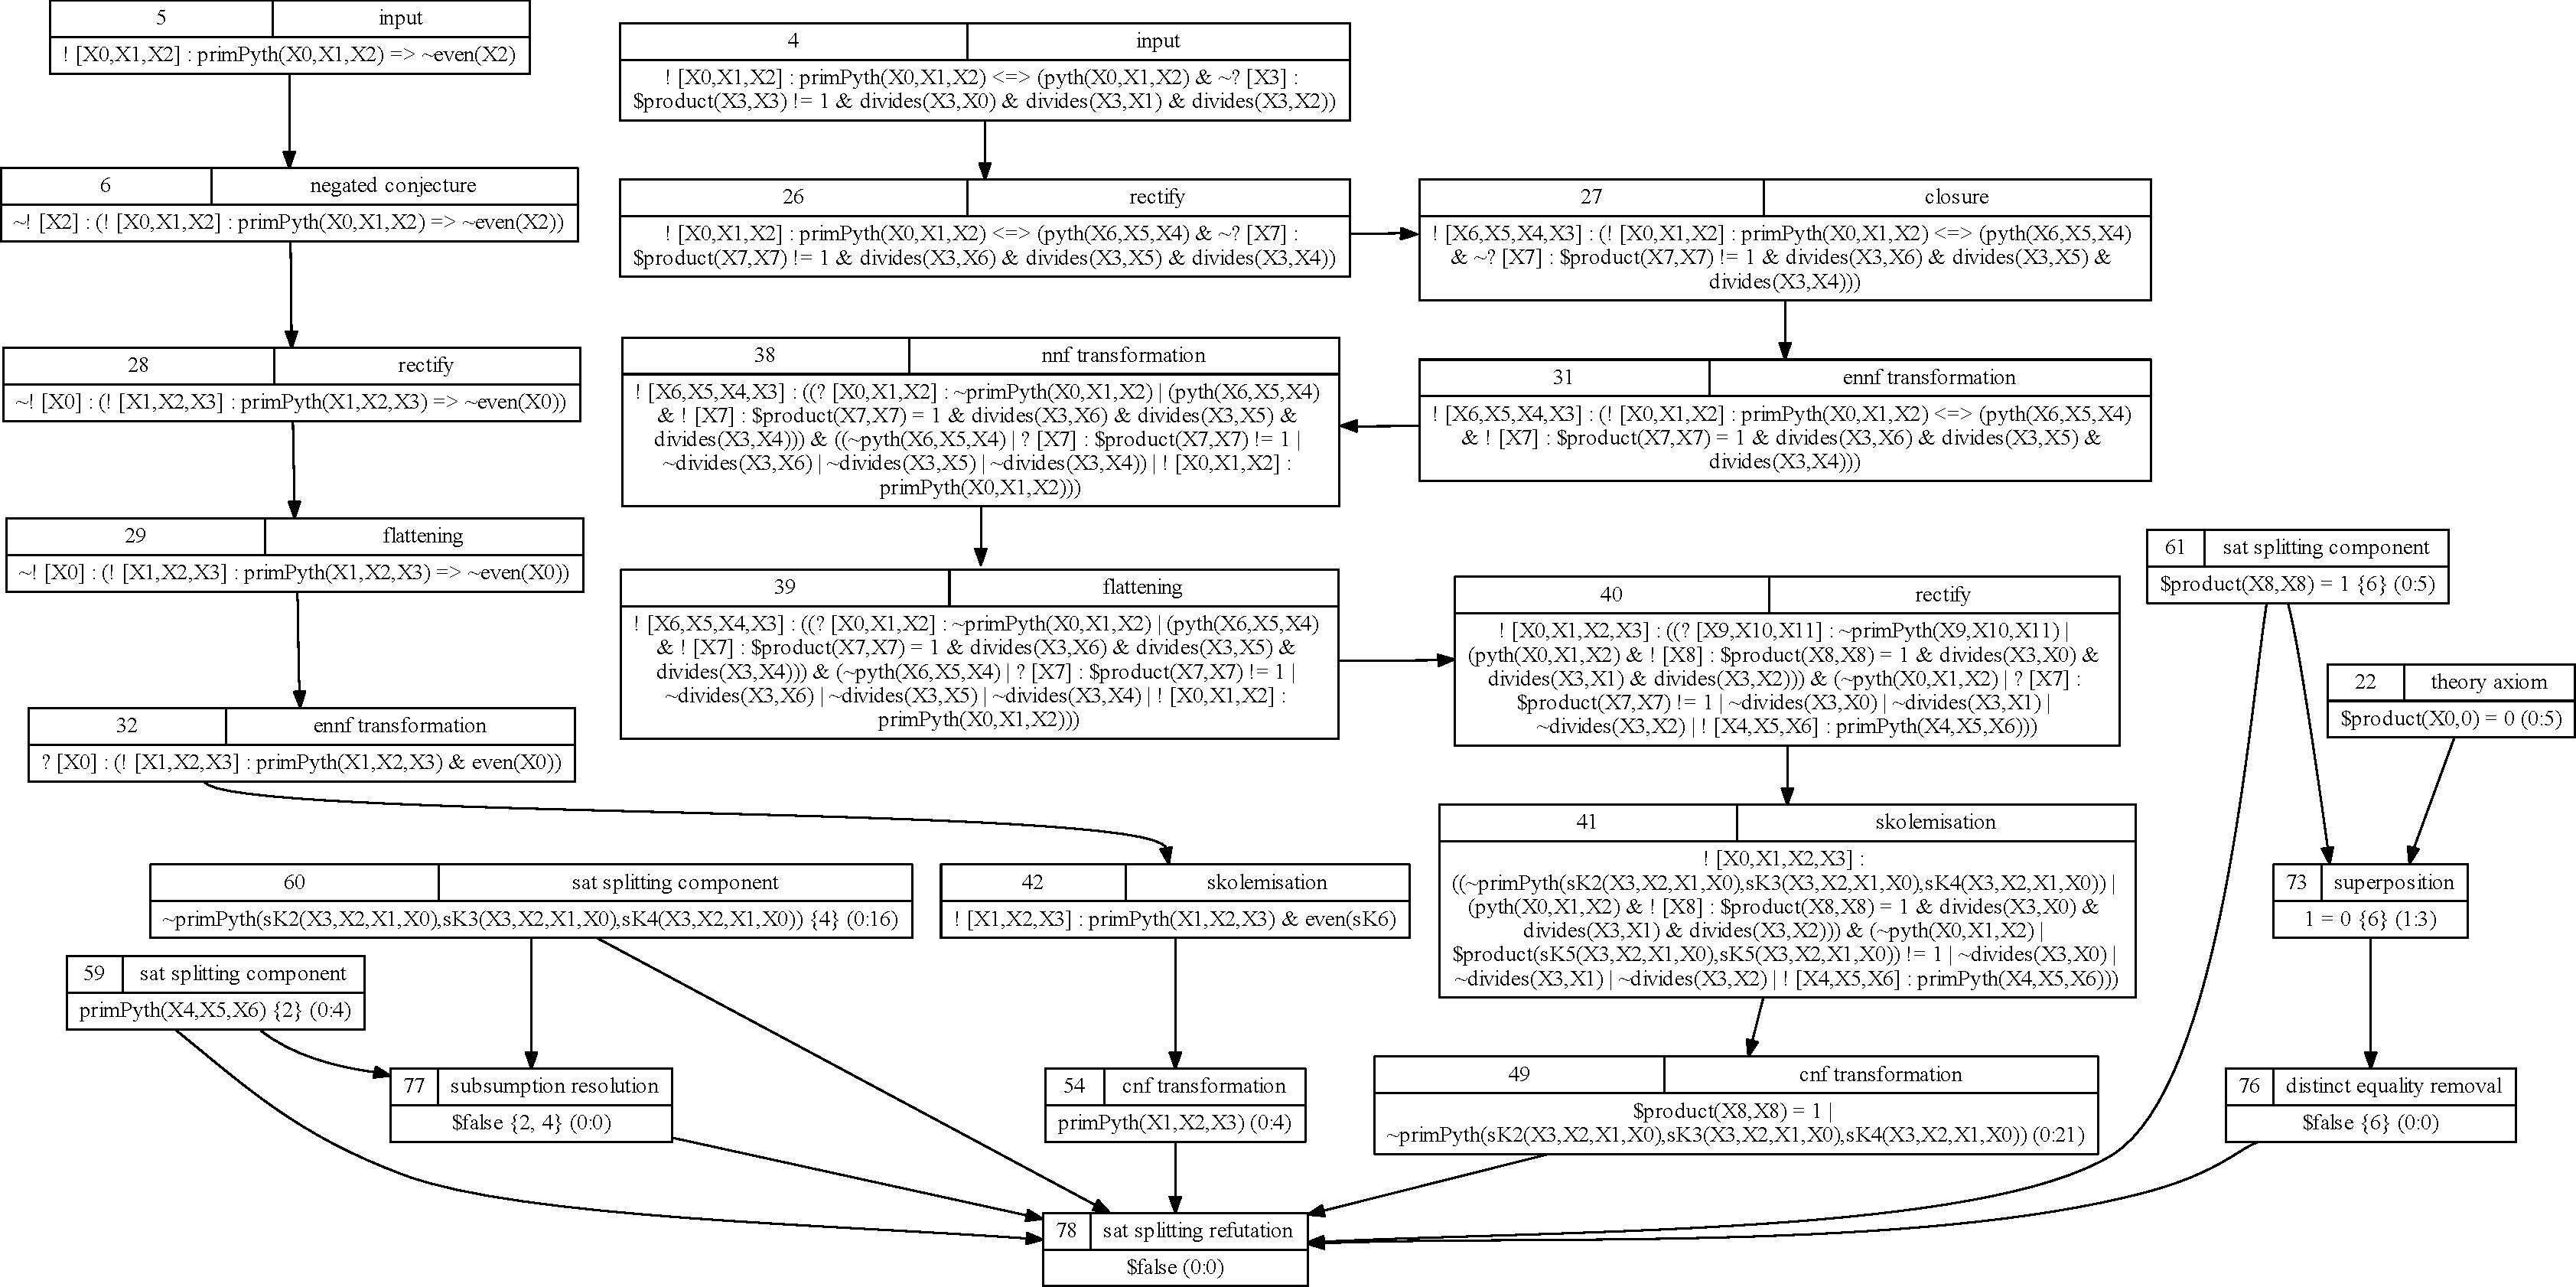
\includegraphics[width=.9\paperwidth]{./graphics/pytriple.pdf}}
	\caption{Graphdarstellung des Beweis-DAG.}
	\label{fig:pytripleproof}
\end{figure}

\end{document}

